\documentclass[12pt]{article}
\usepackage[a4paper]{geometry}
\usepackage[utf8]{inputenc}
\usepackage{fancyhdr}
\usepackage{lastpage}
\usepackage{graphicx, wrapfig, subcaption, setspace, booktabs}
\usepackage{graphicx}
\usepackage[T1]{fontenc}
\usepackage[font=small, labelfont=bf]{caption}
\usepackage[protrusion=true, expansion=true]{microtype}
\usepackage[english]{babel}
\usepackage{sectsty}
\usepackage{url, lipsum}
\usepackage[T1]{fontenc}
\usepackage{icomma}
\usepackage{siunitx}
\usepackage{ragged2e}
\usepackage{amsmath}
\usepackage{comment}
\usepackage{enumerate}
\usepackage{anysize}
\usepackage{graphicx}
\usepackage{amssymb}
\usepackage{apacite}
\bibliographystyle{apacite}
\newcommand{\HRule}[1]{\rule{\linewidth}{#1}}
\onehalfspacing
\setcounter{tocdepth}{5}
\setcounter{secnumdepth}{5}
\usepackage[utf8]{inputenc}
\usepackage{amssymb}
\usepackage{graphicx}
\usepackage{amsmath}
\onehalfspacing
\setcounter{tocdepth}{5}
\setcounter{secnumdepth}{5}
\usepackage{hyperref}

%-------------------------------------------------------------------------------
% HEADER & FOOTER
%-------------------------------------------------------------------------------


\begin{comment}
-Udledninger
$$
\begin{aligned}
\end{aligned}
$$

-Opgavetekst
\begin{figure}[H]
\includegraphics[width=0.5\textwidth]{"path"}
\end{figure} 


-Opgave billede med tekst
\begin{figure}[H]
\caption{"Billedtekst"}
\includegraphics[width=0.5\textwidth]{"path"}
\end{figure} 

-Værdier
$\\
$


\end{comment}
\begin{document}

\begin{titlepage}

\title{ \normalsize 
		%\begin{figure}
        \begin{center}
        
\includegraphics[height=6cm]{Logo.jpg}
        \end{center}
       % \end{figure}
        \LARGE \textsc{\textbf{Universidad De Sonora}} \\ \bigskip
		\Large División de Ciencias Exactas y Naturales \\
        Licenciatura en Física \\ \bigskip
        \bigskip
        Física Computacional I
		\\ [0.1cm]  
		\HRule{2pt} \\
		\Large \textbf{{Actividad 12}} \\
        \textit{\textbf{"Solución Numérica de Ecuaciones Diferenciales Parciales."}}
		\HRule{2pt} \\
		\normalsize \vspace*{0.001\baselineskip}}
        
\date{\bigskip \Large  \hspace*{\fill} Hermosillo, Sonora a abril 26 de 2021}

        
\author{
		\Large\textbf{Ismael Espinoza Arias} \\ \bigskip
        \\ \bigskip
       \Large Profesor Carlos Lizárraga Celaya}
       \end{titlepage}
       \maketitle
       
       
%-----------------------------------------------------------


\section*{Síntesis de sobres las ecuaciones diferenciales, utilizando el método de "Diferencias Finitas"}

La presente Actividad se centra en sintetizar y fundamentar las últimas tres actividades realizadas, sobre solución numérica de Ecuaciones Diferenciales Parciales utilizando el Método de Diferencias Finitas.


%-------------------------------------------------------------


\section{Ecuaciones diferenciales parciales}

En matemáticas , una ecuación diferencial parcial ( PDE ) es una ecuación que impone relaciones entre las diversas derivadas parciales de una función multivariable .

A menudo se piensa que la función es una "desconocida" que se debe resolver, de manera similar a como se piensa que x es un número desconocido, que se debe resolver, en una ecuación algebraica como $x^{2} - 3x + 2 = 0$. Sin embargo, generalmente es imposible escribir fórmulas explícitas para soluciones de ecuaciones diferenciales parciales. En consecuencia, existe una gran cantidad de investigación matemática y científica moderna sobre métodos para aproximar numéricamente soluciones de ciertas ecuaciones diferenciales parciales utilizando computadoras. Las ecuaciones diferenciales parciales también ocupan un gran sector de la investigación matemática pura., en el que las preguntas habituales son, en términos generales, sobre la identificación de características cualitativas generales de las soluciones de varias ecuaciones diferenciales parciales.

\begin{center}
    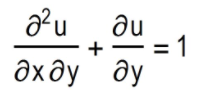
\includegraphics[height=3cm]{EDP.png}
\end{center}


%-------------------------------------------------------------


\section{Métodos numéricos para ecuaciones diferenciales parciales}

Los métodos numéricos para ecuaciones diferenciales parciales es la rama del análisis numérico que estudia la solución numérica de ecuaciones diferenciales parciales (PDE).

    \subsection{Método de diferencias finitas}
    
    En este método, las funciones se representan por sus valores en ciertos puntos de la cuadrícula y las derivadas se aproximan a través de diferencias en estos valores.
    
     \begin{center}
         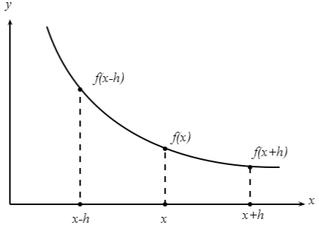
\includegraphics[height=8cm]{DF.png}
     \end{center}
    
    \subsection{Método de líneas}
    
    El método de líneas (MOL, NMOL, NUMOL) es una técnica para resolver ecuaciones diferenciales parciales (PDE) en la que todas las dimensiones menos unas están discretizadas. MOL permite utilizar métodos y software estándar de propósito general, desarrollados para la integración numérica de ecuaciones diferenciales ordinarias (ODE) y ecuaciones algebraicas diferenciales (DAE). Se ha desarrollado una gran cantidad de rutinas de integración a lo largo de los años en muchos lenguajes de programación diferentes, y algunas se han publicado como recursos de código abierto.

El método de líneas se refiere más a menudo a la construcción o análisis de métodos numéricos para ecuaciones diferenciales parciales que procede primero discretizando las derivadas espaciales solamente y dejando la variable de tiempo continua. Esto conduce a un sistema de ecuaciones diferenciales ordinarias al que se puede aplicar un método numérico para ecuaciones ordinarias de valor inicial. El método de las líneas en este contexto se remonta al menos a principios de la década de 1960.

     \begin{center}
         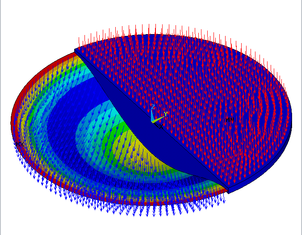
\includegraphics[height=8cm]{ML.png}
     \end{center}


   \subsection{Método de elementos finitos}
   
   El método de los elementos finitos (FEM) es una técnica numérica para encontrar soluciones aproximadas a problemas de valores de frontera para ecuaciones diferenciales. Utiliza métodos variacionales (el cálculo de variaciones) para minimizar una función de error y producir una solución estable. De manera análoga a la idea de que conectar muchas líneas rectas pequeñas puede aproximarse a un círculo más grande, FEM abarca todos los métodos para conectar muchas ecuaciones de elementos simples en muchos subdominios pequeños, denominados elementos finitos, para aproximar una ecuación más compleja en un dominio más grande.
   
   \begin{center}
         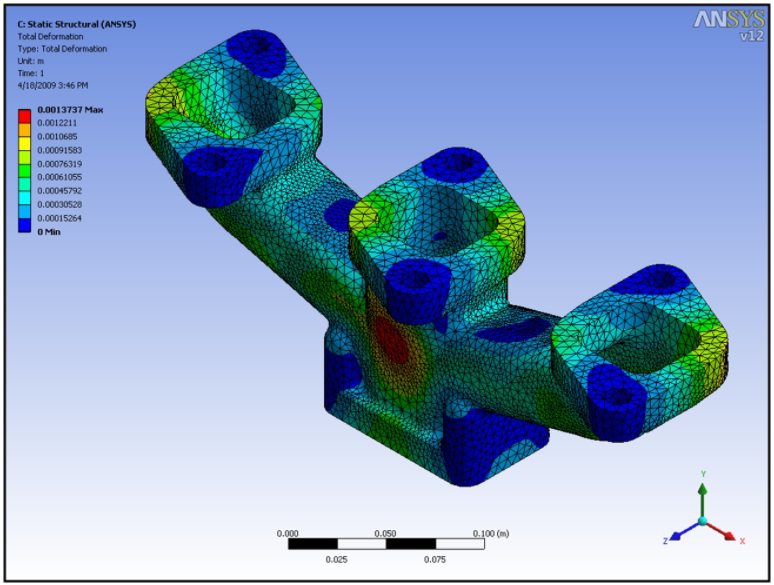
\includegraphics[height=8cm]{MEF.png}
   \end{center}
   
   
   \subsection{Método de discretización de gradiente}
   
   El método de discretización de gradiente (GDM) es una técnica numérica que abarca algunos métodos estándar o recientes. Se basa en la aproximación separada de una función y de su gradiente. Las propiedades centrales permiten la convergencia del método para una serie de problemas lineales y no lineales, y por lo tanto todos los métodos que entran en el marco GDM (elemento finito conforme y no conforme, elemento finito mixto, diferencia finita mimética) heredan estas propiedades de convergencia.
   
   \begin{center}
         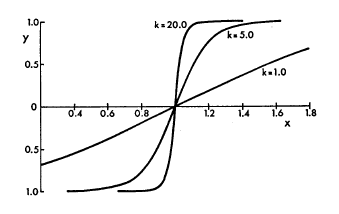
\includegraphics[height=8cm]{MDG.png}
   \end{center}
   
   
   \subsection{Método de volumen finito}
   
   El método de volumen finito es un método para representar y evaluar ecuaciones diferenciales parciales en forma de ecuaciones algebraicas. De manera similar al método de diferencias finitas o al método de elementos finitos, los valores se calculan en lugares discretos en una geometría mallada. "Volumen finito" se refiere al pequeño volumen que rodea cada punto de nodo en una malla. En el método de volumen finito, las integrales de volumen en una ecuación diferencial parcial que contienen un término de divergencia se convierten en integrales de superficie, usando el teorema de divergencia. Estos términos luego se evalúan como flujos en las superficies de cada volumen finito. Debido a que el flujo que ingresa a un volumen dado es idéntico al que sale del volumen adyacente, estos métodos son conservadores. Otra ventaja del método de volumen finito es que se formula fácilmente para permitir mallas no estructuradas. El método se utiliza en muchos paquetes de dinámica de fluidos computacional.
   
   \begin{center}
         \includegraphics[height=6cm]{vf.png}
   \end{center}
   
   
   \subsection{Método espectral}
   
   Los métodos espectrales son técnicas utilizadas en matemáticas aplicadas y computación científica para resolver numéricamente ciertas ecuaciones diferenciales, que a menudo implican el uso de la transformada rápida de Fourier. La idea es escribir la solución de la ecuación diferencial como una suma de ciertas "funciones base" (por ejemplo, como una serie de Fourier, que es una suma de sinusoides) y luego elegir los coeficientes en la suma que mejor satisfagan el diferencial. ecuación.

Los métodos espectrales y los métodos de elementos finitos están estrechamente relacionados y se basan en las mismas ideas; la principal diferencia entre ellos es que los métodos espectrales usan funciones de base que son distintas de cero en todo el dominio, mientras que los métodos de elementos finitos usan funciones de base que son distintas de cero solo en subdominios pequeños. En otras palabras, los métodos espectrales adoptan un enfoque global, mientras que los métodos de elementos finitos utilizan un enfoque local. En parte por esta razón, los métodos espectrales tienen excelentes propiedades de error, siendo la llamada "convergencia exponencial" la más rápida posible, cuando la solución es fluida. Sin embargo, no se conocen resultados de captura de choque espectral de dominio único tridimensional. En la comunidad de elementos finitos, un método en el que el grado de los elementos es muy alto o aumenta a medida que el parámetro de cuadrícula h disminuye a cero se denomina a veces método de elementos espectrales.

   
   \begin{center}
         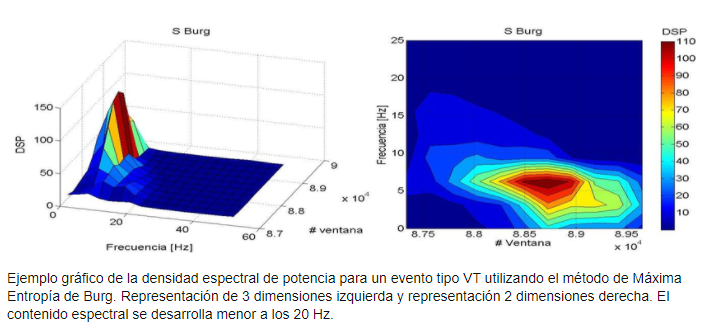
\includegraphics[height=6cm]{ME.png}
   \end{center}
   
   
  \subsection{Métodos sin malla}
   
  Los métodos sin malla no requieren una malla que conecte los puntos de datos del dominio de simulación. Los métodos sin malla permiten la simulación de algunos tipos de problemas que de otro modo serían difíciles, a costa de tiempo de cálculo y esfuerzo de programación adicionales.

   \begin{center}
         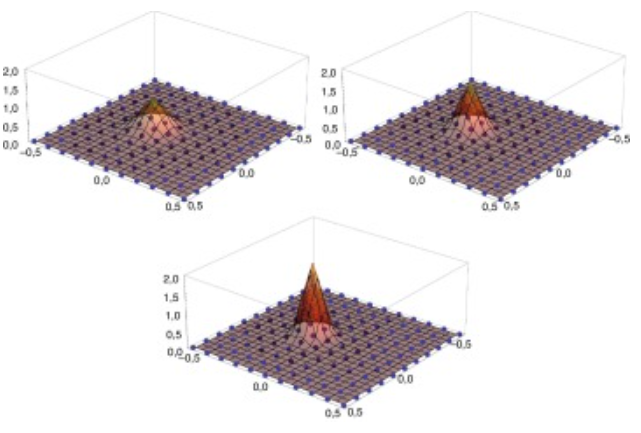
\includegraphics[height=6cm]{MSM.png}
   \end{center}
   

\subsection{Métodos de descomposición de dominios}
   
  Los métodos de descomposición de dominios resuelven un problema de valor límite dividiéndolo en problemas de valor límite más pequeños en subdominios e iterando para coordinar la solución entre subdominios adyacentes. Se utiliza un problema general con una o pocas incógnitas por subdominio para coordinar aún más la solución entre los subdominios a nivel mundial. Los problemas en los subdominios son independientes, lo que hace que los métodos de descomposición de dominios sean adecuados para la computación en paralelo. Los métodos de descomposición de dominios se utilizan normalmente como prea condicionadores para los métodos iterativos del espacio de Krylov, como el método de gradiente conjugado o GMRES.

   \begin{center}
         \includegraphics[height=10cm]{TKM.png}
   \end{center}
   
   
\subsection{Métodos de redes múltiples}
   
  Los métodos de cuadrícula múltiple (MG) en análisis numérico son un grupo de algoritmos para resolver ecuaciones diferenciales usando una jerarquía de discretizaciones. Son un ejemplo de una clase de técnicas llamadas métodos de multirresolución, muy útiles en (pero no limitado a) problemas que exhiben múltiples escalas de comportamiento. Por ejemplo, muchos métodos de relajación básicos exhiben diferentes tasas de convergencia para componentes de longitud de onda corta y larga, lo que sugiere que estas diferentes escalas deben tratarse de manera diferente, como en un enfoque de análisis de Fourier para redes múltiples. [7]Los métodos MG se pueden utilizar como solucionadores y como prea condicionadores.

   \begin{center}
         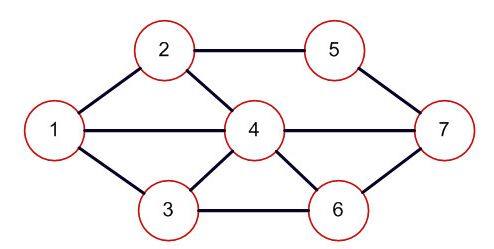
\includegraphics[height=6cm]{MRM.png}
   \end{center}
   

%-------------------------------------------------------------


\section{Método de diferencias finitas}

En el análisis numérico, los métodos de diferencias finitas (FDM) son una clase de técnicas numéricas para resolver ecuaciones diferenciales mediante la aproximación de derivadas con diferencias finitas. Tanto el dominio espacial como el intervalo de tiempo (si corresponde) se discretizan o se dividen en un número finito de pasos, y el valor de la solución en estos puntos discretos se aproxima resolviendo ecuaciones algebraicas que contienen diferencias finitas y valores de puntos cercanos.

Los métodos de diferencias finitas convierten las ecuaciones diferenciales ordinarias (EDO) o las ecuaciones diferenciales parciales (PDE), que pueden ser no lineales, en un sistema de ecuaciones lineales que pueden resolverse mediante técnicas de álgebra matricial. Las computadoras modernas pueden realizar estos cálculos de álgebra lineal de manera eficiente, lo que, junto con su relativa facilidad de implementación, ha llevado al uso generalizado de FDM en el análisis numérico moderno. Hoy en día, FDM es uno de los enfoques más comunes para la solución numérica de PDE, junto con los métodos de elementos finitos.

\begin{center}
    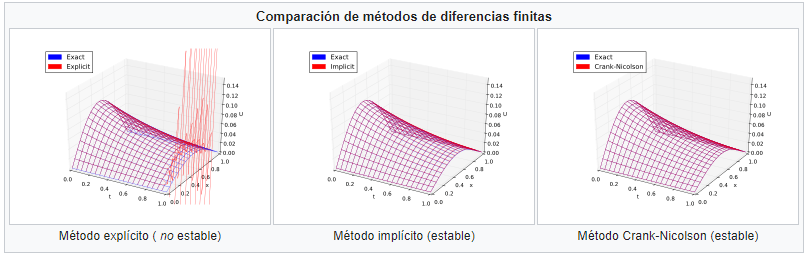
\includegraphics[height=5.5cm]{CMDF.png}
\end{center}


%-------------------------------------------------------------


\section{Ecuación de calor}

La mayoría de los problemas físicos y de ingeniería de importancia práctica están descritos por este tipo de ecuaciones diferenciales, y fundamentalmente por ecuaciones diferenciales de segundo orden. Por ello el tratamiento de las EDP que se desarrollará en lo sucesivo se concentrará sobre ecuaciones lineales de segundo orden. Las ecuaciones diferenciales de segundo orden en derivadas parciales pueden expresarse de forma general como: 

\begin{center}
    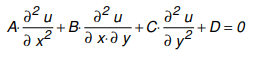
\includegraphics[height=2cm]{ED.png}\\
\end{center}

Para resolver esta ecuación hay que tener en cuenta la distribución inicial de temperaturas en el cuerpo y las condiciones de contorno. Se deduce también, la ecuación de la conducción del calor cuando el cuerpo genera internamente calor por algún procedimiento.

n matemáticas una ecuación en derivadas parciales (a veces abreviada como EDP) es aquella ecuación diferencial cuyas incógnitas son funciones de diversas variables independientes, con la peculiaridad de que en dicha ecuación figuran no solo las propias funciones sino también sus derivadas. Tienen que existir funciones de por lo menos dos variables independientes.1. O bien una ecuación que involucre una función matemática ${\displaystyle u}u$ de varias variables independientes x, y, z, …, y las derivadas parciales de u respecto de esas variables. Las ecuaciones en derivadas parciales se emplean en la formulación matemática de procesos de la física y otras ciencias que suelen estar distribuidos en el espacio y el tiempo. Problemas típicos son la propagación del sonido o del calor, la electrostática, la electrodinámica, la dinámica de fluidos, la elasticidad, la mecánica cuántica y muchos otros. Se las conoce también como ecuaciones diferenciales parciales. Participaron, al inicio, en su estudio los franceses d'Alembert, Fourier, matemáticos de la época napoleónica.

Resolveremos por el método de diferencias finitas la Ecuación del Calor en una dimensión para la temperatura u(t,x), dada una condición inicial y 2 condiciones a la frontera. Por ejemplo una barra de cobre de longitud L=1 (térmicamente aislada en las paredes), y los extremos pueden estar térmicamente aislados, o estar a cierta temperatura fija, o estar libres para que el calor escape.

\begin{center}
    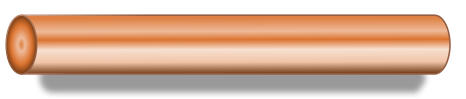
\includegraphics[height=2cm]{EC.png}
\end{center}

Por ejemplo la Ecuación del Calor para una barra de longitud 1, con temperatura fija de 0ºC en los extremos (en contacto con una barra de hielo), y habiendo una distribución de temperatura inicial dentro de la barra descrita por la función f(x). 

\begin{center}
    $U_{t}(x,t) = KU_{xx}(x,t)$\\
    $U(0,t) = U(1,t) = 0$\\
    $U(x,0) = f(x)$\\
\end{center}

\subsection{Importación de bibliotecas}
Empezamos importando nuestras bibliotecas, el primer paso para empezar con cualquier actividad.

\begin{center}
    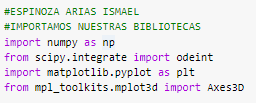
\includegraphics[height=4cm]{Bibliotecas.png}
\end{center}
 
 Donde podemos ver que las bibliotecas utilizadas, son numpy, scipy, matplotlib, toolkits, ect. Donde nos ayudaran a resolver nuestro siguiente problema.


%-----------------------------------------------------------


\subsection*{Realización de la actividad}
Ahora para la actividad, vamos a definir nuestros valores y resolver la ecuación del calor usando ecuaciones diferenciales parciales.

%--------------------------1---------------------------------

\subsection{Ejercicio 1}

Para el caso $a)$ tenemos una barra metálica de longitud $L = 10$, y coeficiente de difusión  $k = 100$ . Condición inicial (Temperatura dentro de la barra): $u(x,0) = 0$. Condiciones a la frontera: $u(0,t) = 10, u(L,t) = 0$. Realice los cálculos hasta alcanzar el equilibrio térmico.

\begin{center}
    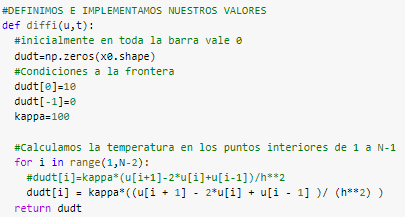
\includegraphics[height=8cm]{E1 (1).png}
\end{center}

Relizando las operaciones correspondientes, llegamos a la gráfica siguiente:

\begin{center}
    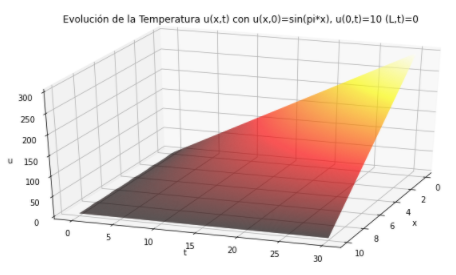
\includegraphics[height=8cm]{Grafica1.png}
\end{center}


Para el caso $b)$ tenemos un material de longitud $L=10$ con coeficiente de difusión térmica $\kappa=0.25$ Condición inicial u(x,0)=20. Condiciones a la frontera: u(0,t)=(20 + 10 sin(pi*t/12), u(L,t)=20. Realice los cálculos para t=(0,48) Pueden ajustar los parámetros para ver cómo cambia la temperatura dentro del cuerpo.

\begin{center}
    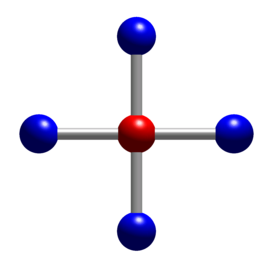
\includegraphics[height=8cm]{E2.png}
\end{center}

Relizando las operaciones correspondientes, llegamos a la gráfica siguiente:

\begin{center}
    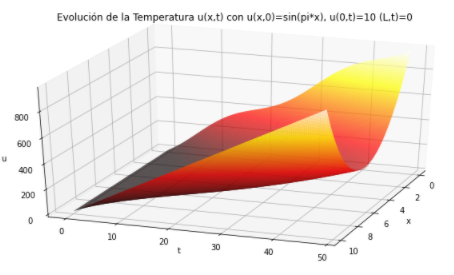
\includegraphics[height=8cm]{Grafica2.png}
\end{center}


Para el caso $c)$ Implementamos la diferencias finitas para esta ocasión.

\begin{center}
    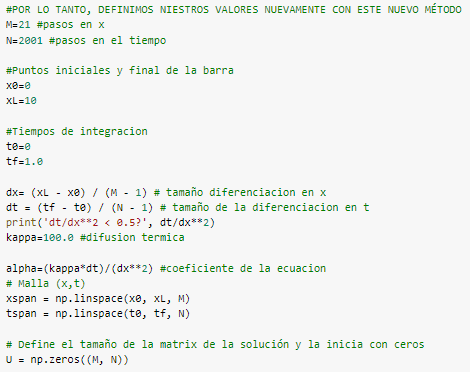
\includegraphics[height=10cm]{E3.png}
\end{center}

Relizando las operaciones correspondientes, llegamos a la gráfica siguiente:

\begin{center}
    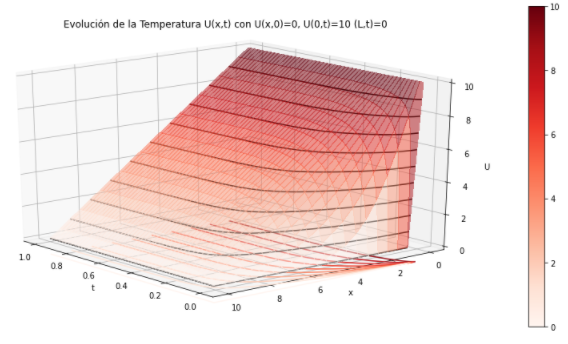
\includegraphics[height=8cm]{Grafica3.png}
\end{center}


Para el caso $d)$ Implementamos la diferencias finitas para esta ocasión.

\begin{center}
    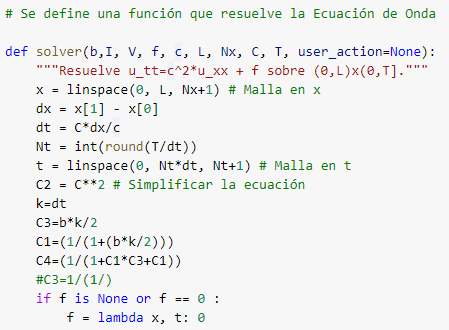
\includegraphics[height=10cm]{E4.png}
\end{center}

Relizando las operaciones correspondientes, llegamos a la gráfica siguiente:

\begin{center}
    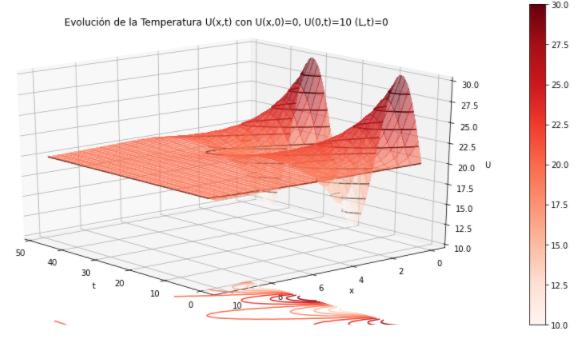
\includegraphics[height=8cm]{Grafica4.png}
\end{center}

%-----------------------------------------------------------

\subsection{Ejercicio 2}

Variaciones de la Temperatura en el Suelo. La superficie de la Tierra recibe radiación solar durante el día. Esta Energía la transforma en calor, y cambia la temperatura dentro del suelo. Por la noche al no recibir radiación solar la emite a la atmósfera. 

Si suponemos que la temperatura del suelo varía con la profundidad, podemos suponer que tenemos un problema unidimensional, siendo el eje $x$ la dirección hacia dentro del suelo.

A cierta profundidad $x=L$, suponemos que la temperatura ya no cambia, es decir $\partial u/\partial x = 0$ (Condición de Neumann).

Supondremos que la variación de la temperatura en la superficie terrestre varía como 

\begin{equation*}
u(0,t) = u_0 + u_a \sin (\frac{2\pi t}{P})
\end{equation*}

donde $u_0$ es la inical temperatura promedio del suelo y $u_a$ es la temperatura del aire. La constante $P$ es el periodo de variación diaria de temperatura $P=24 h=86,400 s$.

En este caso la constante de difusión de calor es $\kappa = 1.0 \times 10^{-6}$. El tiempo será medido en segundos. 

Usando la Ecuación de Calor, determina numéricamente  la variación del perfil de temperatura dentro del suelo, por ejemplo para Hermosillo en estos días supongamos que $u_0=15^{o}C$, $u_a= 20^{o}C$. Realiza una simulación de al menos 48 horas. 

\begin{center}
    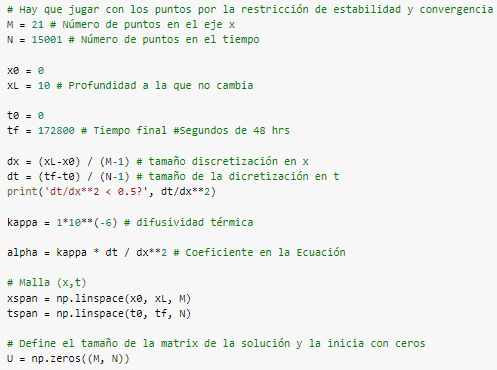
\includegraphics[height=8cm]{E5.png}
\end{center}

Relizando las operaciones correspondientes, llegamos a la gráfica siguiente:

\begin{center}
    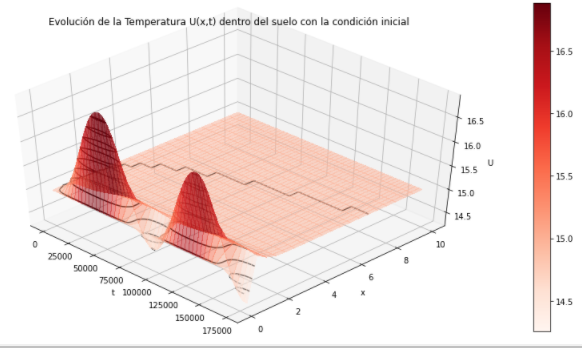
\includegraphics[height=8cm]{Grafica5.png}
\end{center}

\begin{center}
    Repertorio en Githuib:
    
    \url{https://github.com/IsmaelEA2020/Fisica-computacional/tree/main/Actividad10}
\href{http://www.latex-project.org/}{Actividad 10}

\end{center}




%-------------------------------------------------------------


\section{Ecuación de onda}

Consideremos una perturbación, generada en una cuerda, que viaja hacia
la derecha con una rapidez constante u. Si convenimos en denotar por x
a las diferentes posiciones a lo largo de la dirección de propagación de la
perturbación y por y a las posiciones perpendiculares a ésta, la forma de la
perturbación quedará descrita por una función y = f(x,t). Si durante la propagación
de la perturbación no existe disipación de energía, la forma y el tamaño de la
perturbación no cambiarán a medida que ésta se desplaza. (En particular, la
propagación de la luz en el espacio vacío cumple con este requisito.) En tal caso
se debe cumplir necesariamente que:

\begin{center}
    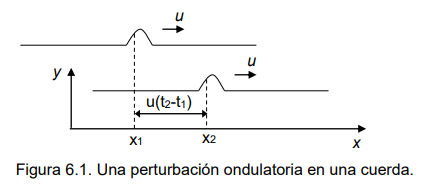
\includegraphics[height=6cm]{E1.png}
\end{center}

en donde $x2 = x1 + u(t2 - t1), ya que u(t2 - t1)$ es la distancia que ha avanzado la
perturbación en el intervalo t2 - t1. Este requisito se cumple si la función que
describe a la perturbación tiene la forma:

\begin{center}
    $f(x,t) = y(x - ut) $
    
    ya que entonces:
    
    $f(x2,t2) = y(x2 - ut2) = y[x1 + u(t2 - t1)- ut2] = y( x1 - ut1) = f(x1,t1)$
    
\end{center}

La ecuación de onda es una ecuación diferencial parcial de segundo orden en el tiempo y las coordenadas espaciales y tiene la forma

\begin{equation*}
\frac{\partial^2 u}{\partial t^2} = c^2 \left( 
  \frac{\partial^2 u}{\partial x^2} +
  \frac{\partial^2 u}{\partial y^2} +
  \frac{\partial^2 u}{\partial z^2} \right) + f(x,y,z,t)
\end{equation*}

donde $c^{2}$ es la velocidad de propagación de la información. La función $u(x,y,z,t)$ representa la presión en una onda acústica, la intensidad de un campo electromagnético, el desplazamiento respecto a un nivel de referencia como lo puede ser la amplitud de una onda superficial en la superficie del agua o el desplazamiento respecto a la horizontal de una cuerda vibrante. 

En una dimensión, por ejemplo el caso de una cuerda vibrante, la Ecuación de Onda se simplifica a 

\begin{equation*}
\frac{\partial^2 u}{\partial t^2} = c^2 \left( 
  \frac{\partial^2 u}{\partial x^2}
   \right) + f(x,t) \qquad x \in (0,L], t \in (0,T]
\end{equation*}

Requerimos definir 4 condiciones: 2 iniciales (derivada de segundo orden en t) y 2 a la frontera (segundo orden en el espacio), para encontrar la solución.

\begin{eqnarray*}
u(x,0) & = & I(x) \\
\frac{\partial}{\partial t} u(x,0) & = & 0 \\
u(0,t) & = & 0 \\
u(L,t) & = & 0 \\
\end{eqnarray*}

Se requiere también especificar el valor de la constante $c$ y la función $I(x)$.

\section{Solución de la Ecuación de Onda en una dimensión por el Método de Diferencias Finitas.}

Podemos comenzar aproximando las segundas derivadas por diferencias finitas centradas de segundo orden.

Si $h$ es el incremento en la dirección $x=\Delta x$ y $k=\Delta t$ es el incremento en el tiempo. Entonces en un punto de la malla discreta $(x,t)$ tendremos

\begin{equation*}
\frac{u(x,t+k) -2u(x,t) + u(x,t-k)}{k^2} = c^2
\frac{u(x+h,t) -2u(x,t) + u(x-h,t)}{h^2}
\end{equation*}

La ecuación anterior define un esténcil computacional de 5 puntos y se respresenta como:

\begin{center}
    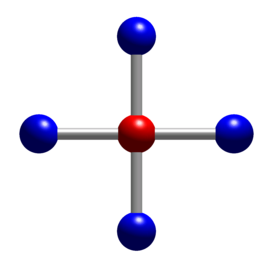
\includegraphics[height=6cm]{E2.png}
\end{center}


%-----------------------------------------------------------


\subsection{Importación de bibliotecas}
Empezamos importando nuestras bibliotecas, el primer paso para empezar con cualquier actividad.

\begin{center}
    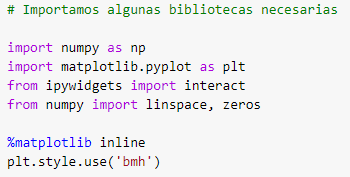
\includegraphics[height=6cm]{bibliotecas1.png}
\end{center}
 
 Donde podemos ver que las bibliotecas utilizadas, son numpy, scipy, matplotlib, toolkits, ect. Donde nos ayudaran a resolver nuestro siguiente problema.


%-----------------------------------------------------------


\subsection{Realización de la actividad}
Ahora para la actividad, vamos a definir nuestros valores y resolver la ecuación de onda usando ecuaciones diferenciales parciales.

\begin{center}
    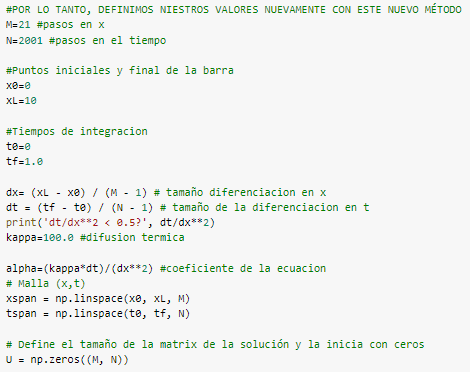
\includegraphics[height=10cm]{E3.png}
    \includegraphics[height=10cm]{cuerda.png}
\end{center}

 

%--------------------------1---------------------------------


\subsection{Ejercicio 1}

Modifique el algoritmo de diferencias finitas empleado anteriormente y resuelva la ecuación de onda amortiguada en una dimensión, dada por la ecuación

\begin{equation*}
\frac{\partial^2 u}{\partial t^2} + 
 b \frac{\partial u}{\partial t}
 = c^2 \left( 
  \frac{\partial^2 u}{\partial x^2}
   \right) \qquad x \in (0,L], t \in (0,T]
\end{equation*}

donde $b \ge 0 $ y $c$ son constantes. 

Se proporcionan las condiciones iniciales y a la frontera para encontrar la solución.

\begin{eqnarray*}
u(x,0) & = & I(x) \\
\frac{\partial}{\partial t} u(x,0) & = & 0 \\
u(0,t) & = & 0 \\
u(L,t) & = & 0 \\
\end{eqnarray*}

Utilice diferencias finitas centradas de segundo orden para aproximar la primer derivada $\partial u/\partial t$.

\begin{equation*}
\frac{\partial}{\partial t} u(x,t) \approx \frac{u(x,t+k) - u(x,t-k)}{2k}
\end{equation*}

Suponga las mismas características del ejemplo presentado anteriormente $L=10$, $c=100$m/s, $t=(0,0.25)$, y coeficiente de amortiguamiento $b=0.5$ con condiciones iniciales $u(x,0) = x(1-x)$ y $\partial u(x,0) / \partial t = 0$ y condiciones a la frontera $u(0,t)=u(L,t)=0$. 

Realizamos la resolución de nuestro ejercicio.

\begin{center}
    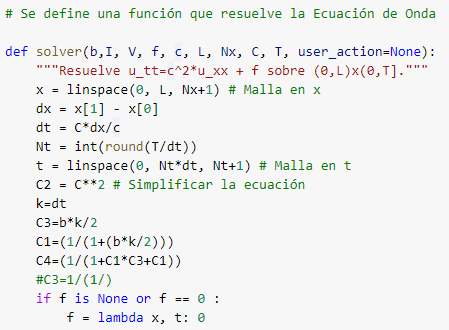
\includegraphics[height=10cm]{E4.png}
    
    Donde llegamos al siguiente resultado:
    
    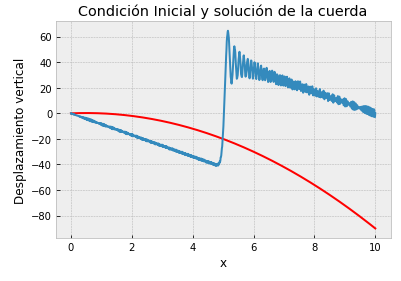
\includegraphics[height=8cm]{Ejercicio1.png}
\end{center}




%---------------------------2--------------------------------


\subsection{Ejercicio 2}

Haga el desarrollo del algoritmo de diferencias finitas centradas para resolver la ecuación de onda en 1 dimensión si se tiene un término de forzamiento $f(x,t)$

\begin{equation*}
\frac{\partial^2 u}{\partial t^2} = c^2 \left( 
  \frac{\partial^2 u}{\partial x^2}
   \right) + f(x,t) \qquad x \in (0,L], t \in (0,T]
\end{equation*}

Con las condiciones iniciales y a la frontera para encontrar la solución.

\begin{eqnarray*}
u(x,0) & = & I(x) \\
\frac{\partial}{\partial t} u(x,0) & = & 0 \\
u(0,t) & = & 0 \\
u(L,t) & = & 0 \\
\end{eqnarray*}

Realizamos la resolución de nuestro ejercicio.

\begin{center}
    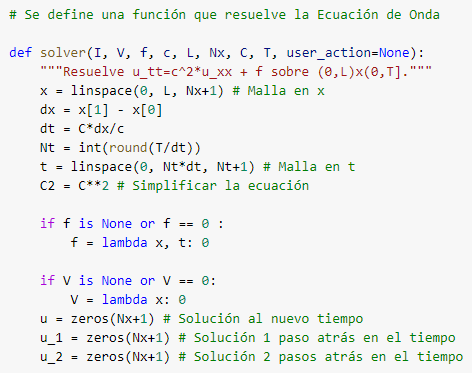
\includegraphics[height=10cm]{Ejercicio2.png}
    
    Donde llegamos al siguiente resultado:
    
    \includegraphics[height=8cm]{Ejercicio2.1.png}
\end{center}


%---------------------------3---------------------------------


\subsection{Ejercicio 3}

Resuelva la Ecuación KdV, para el caso de 2 solitones comenzando en $x01 = 0.25*L$ y $x02 = 0.75*L$, con velocidades $c1=0.75$ y $c2=0.01$ e integre hasta que una de las ondas llegue a la frontera.

Grafique las soluciones como en el ejemplo que se proporcionó.


Realizamos la resolución de nuestro ejercicio.

\begin{center}
    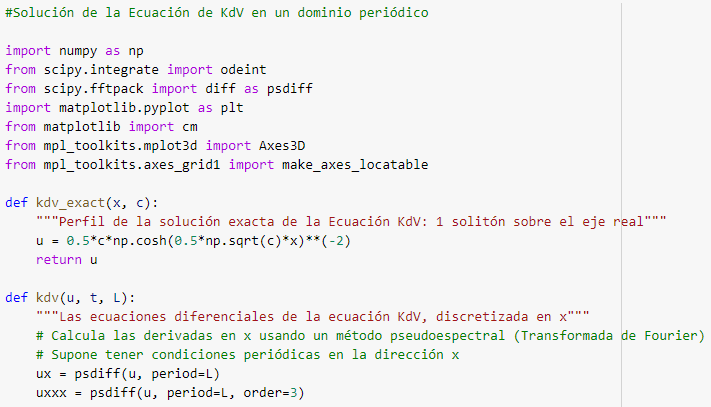
\includegraphics[height=8cm]{Ejercicio3.png}
    
    Donde llegamos al siguiente resultado:
    
    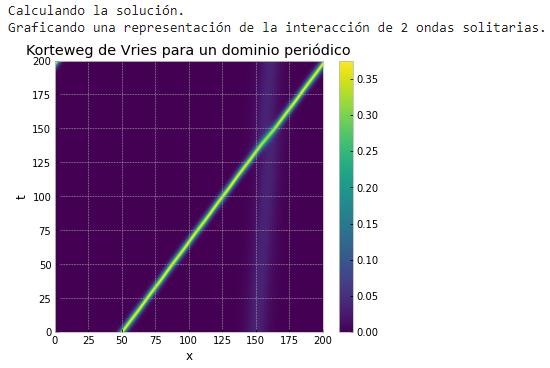
\includegraphics[height=8cm]{Ejercicio3.1.png}
    
     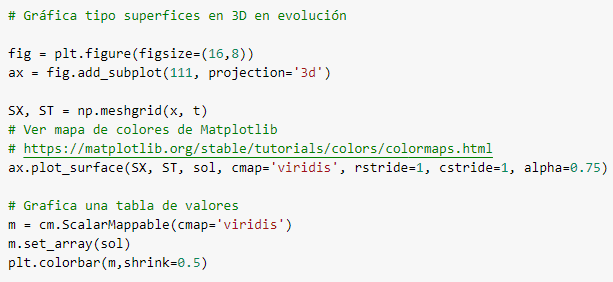
\includegraphics[height=6cm]{Ejercicio3.2.png}
    
    Donde llegamos al siguiente resultado:
    
    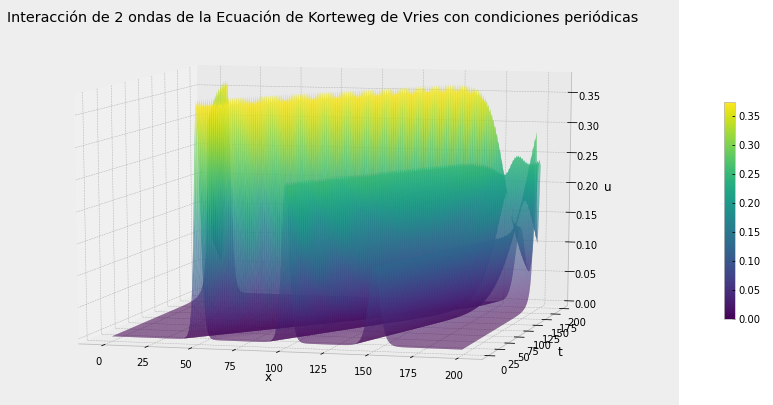
\includegraphics[height=8cm]{Ejercicio3.3.png}
\end{center}


%---------------------------4---------------------------------


\subsection{Ejercicio 4}

Resuelva la Ecuación KdV, para el caso de 3 solitones comenzando en $x01 = 0.25*L$, $x02=0.5*L$, y $x03 = 0.75*L$, con velocidades $c1=0.75$, $c2=0.5$ y $c3=0.25$ e integre hasta que una de las ondas llegue a la frontera.

Grafique las soluciones.

Realizamos la resolución de nuestro ejercicio.

\begin{center}
    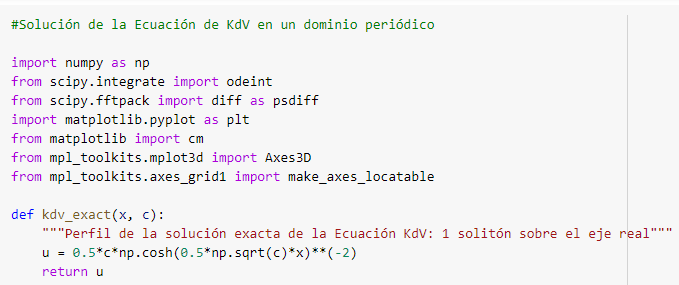
\includegraphics[height=6cm]{Ejercicio4.png}
    
    Donde llegamos al siguiente resultado:
    
    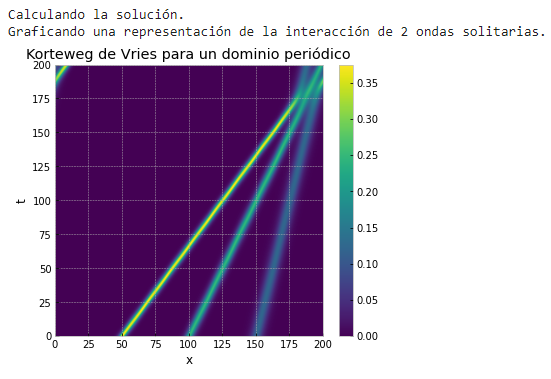
\includegraphics[height=8cm]{Ejercicio4.1.png}
    
     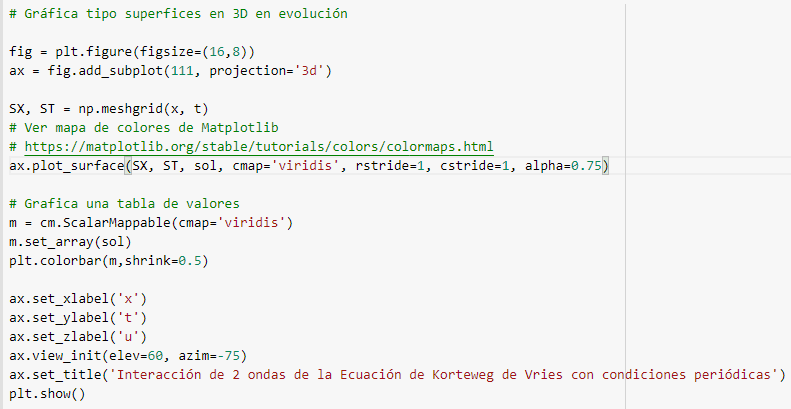
\includegraphics[height=8cm]{Ejercicio4.2.png}
    
    Donde llegamos al siguiente resultado:
    
    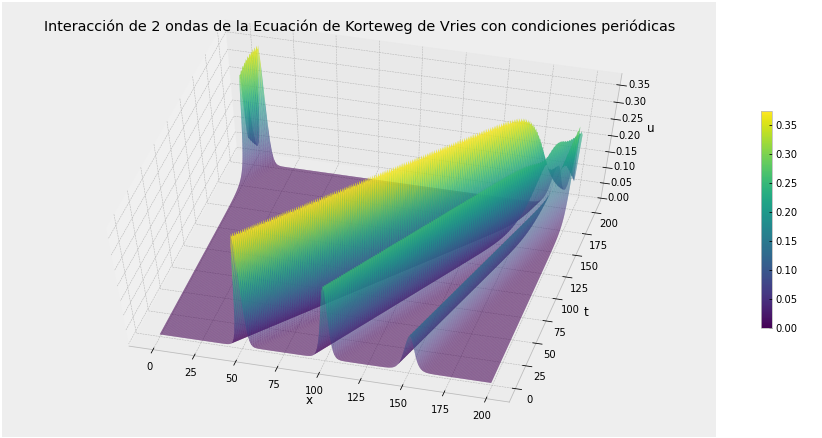
\includegraphics[height=8cm]{Ejercicio4.3.png}
\end{center}


%---------------------------5---------------------------------


\subsection{Ejercicio 5}

En el ejemplo resuleto anterior, se mostró la evolución de la condición inicial 

\begin{equation*}
u_0^{(2,1)}(x,y,0) = sin (\pi x) \sin (\frac{\pi y}{2})
\end{equation*}

mostrando el *modo (1,2)* de oscilación natural de la membrana ([Ver estas animaciones](https://www.acs.psu.edu/drussell/Demos/MembraneSquare/Square.html)). 
 
En este Ejercicio se pide mostrar la evolución del *modo (1,1)*, con la condición inicial 

\begin{equation*}
u_0^{(1,1)}(x,y,0) = \sin (\frac{\pi x}{2}) \sin (\frac{\pi y}{2})
\end{equation*}

\begin{center}
    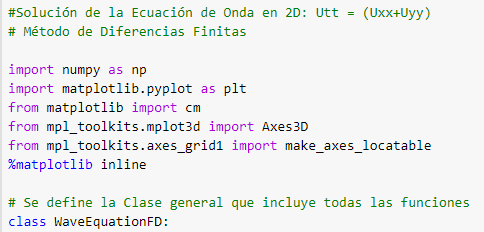
\includegraphics[height=6cm]{Ejercicio5.png}
    
    Donde llegamos a la siguientes gráficas:
    
    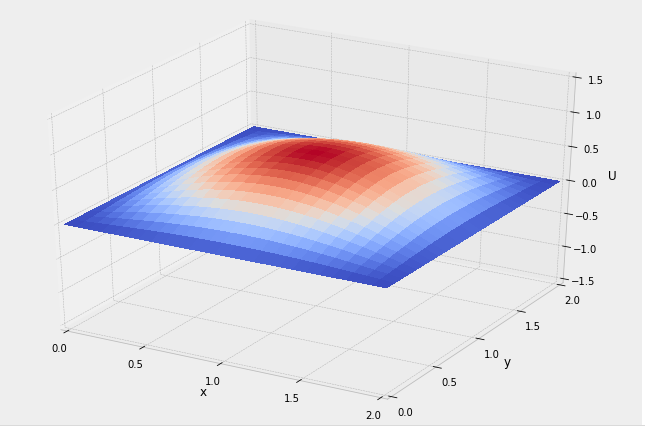
\includegraphics[height=5cm]{Gráfica1.png}
    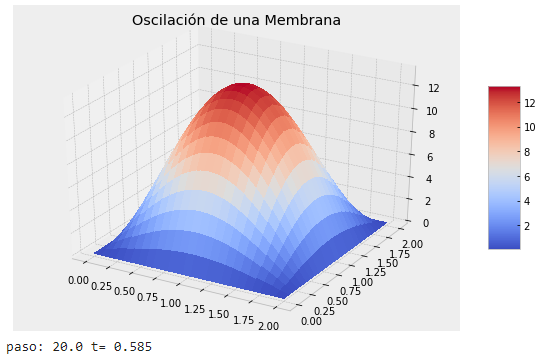
\includegraphics[height=5cm]{Gráfica2.png}
    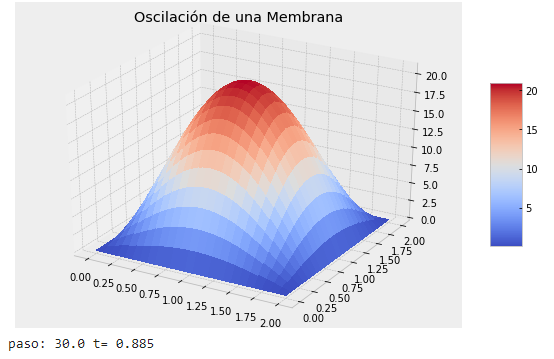
\includegraphics[height=5cm]{Gráfica3.png}
    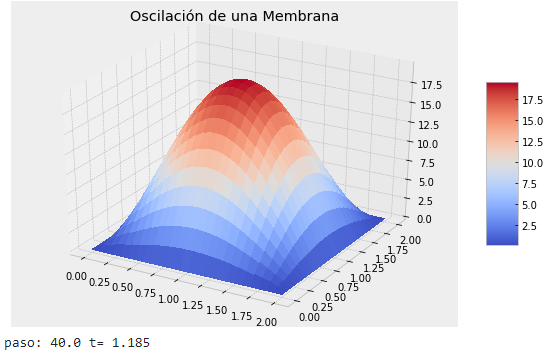
\includegraphics[height=5cm]{Gráfica4.png}
    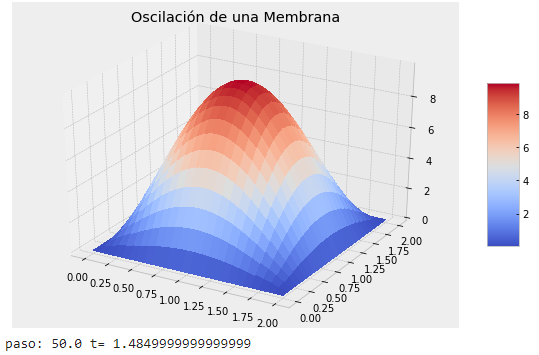
\includegraphics[height=5cm]{Gráfica5.png}
    \includegraphics[height=5cm]{Gráfica6.png}
    \includegraphics[height=5cm]{Gráfica7.png}
    \includegraphics[height=5cm]{Gráfica8.png}
    \includegraphics[height=5cm]{Gráfica9.png}
    \includegraphics[height=5cm]{Gráfica10.png}
    \includegraphics[height=5cm]{Gráfica11.png}
    
\end{center}


%---------------------------6---------------------------------


\subsection{Ejercicio 6}

En el mismo contexto que el problema anterior, muestra la evolución de la superposición *modos (3,1)+ (1,3)* dada la condición inicial

\begin{equation*}
u_0^{(3,1)+(1,3)}(x,y,0) = \sin (\frac{3 \pi x}{2}) \sin (\frac{\pi y}{2}) + \sin (\frac{\pi x}{2}) \sin (\frac{3 \pi y}{2})
\end{equation*}

\begin{center}
    \includegraphics[height=10cm]{Ejercicio6.png}
    
    Donde llegamos a la siguientes gráficas:
    
    \includegraphics[height=5cm]{s1.png}
    \includegraphics[height=5cm]{s2.png}
    \includegraphics[height=5cm]{3.png}
    \includegraphics[height=5cm]{s4.png}
    \includegraphics[height=5cm]{s5.png}
    \includegraphics[height=5cm]{s6.png}
    \includegraphics[height=5cm]{s7.png}
    \includegraphics[height=5cm]{s8.png}
    \includegraphics[height=5cm]{s9.png}
    \includegraphics[height=5cm]{s10.png}
    \includegraphics[height=5cm]{s11.png}

    
\end{center}

\begin{center}
    Repertorio en Githuib:
    
    \url{https://github.com/IsmaelEA2020/Fisica-computacional/tree/main/Actividad11}
\href{http://www.latex-project.org/}{Actividad 11}

\end{center}

%-------------------------------------------------------------


\section{Ecuación de Poisson}

La Ecuación de Poisson es una Ecuación Diferencial Parcial de tipo Elíptico. La Ecuación de Poisson es una generalización de la Ecuación de Laplace. Un caso general de la Ecuación de Laplace es la Ecuación de Helmholtz, que surge de resolver un problema de eigenvalores del operador de Laplace. La Ecuación de Poisson es utilizada en algunos campos de la Física como lo es la teoría de gravitación de Newton, la electrostática, dinámica de fluidos y otros. Uno de los métodos para resolver la Ecuación de Poisson es el método de diferencias finitas. También existen otros métodos para resolver ls Ecuación de Poisson como lo son con el método de elemento finito, el método pseudoespectral, entre otros. 

La ecuación de Poisson es una ecuación diferencial parcial elíptica de amplia utilidad en física teórica . Por ejemplo, la solución a la ecuación de Poisson es el campo potencial causado por una determinada carga eléctrica o distribución de densidad de masa; con el campo de potencial conocido, se puede calcular el campo (fuerza) electrostático o gravitacional. Es una generalización de la ecuación de Laplace , que también se ve con frecuencia en física. La ecuación lleva el nombre del matemático y físico francés Siméon Denis Poisson .

\begin{center}
\includegraphics[height=10cm]{Poisson.png}
\end{center}




%-----------------------------------------------------------


\subsection{Solución de Ecuaciones Diferenciales Parciales de tipo Elíptico.}

\begin{equation*}
- \nabla^2 u(x,y,z) = f(x,y,z) 
\end{equation*}

con distintas condiciones a la frontera:


*   Condiciones de Dirichlet (especificando valores de la función $u$)
*   Condiciones de Neumann (especificando valores de la derivada de la función $u$ perpendicular a la frontera $\partial u/\partial n$).

La Ecuación de Poisson aparece en problemas de campos gravitatorios, campos eléctricos y otros problemas en la Física. 



\begin{equation*}
\nabla^2 u = 0
\end{equation*}

Se busca la solución de la ecuación 

\begin{equation*}
- \nabla^2 u = f
\end{equation*}

dadas las condiciones en la frontera $\Gamma$

\begin{equation*}
u(x,y)_{\Gamma} = g(x,y)
\end{equation*}

No requerimos una condición inicial, pues no hay dependencia en el tiempo. Sólo requerimos conocer los valores a la frontera.

Supongamos que tenemos un dominio rectangular cartesiano $\Gamma = (a,b) \times (c,d)$, sobre el cual generamos una malla 

\begin{eqnarray*}
x_i & = & a + i h_x \quad i={0,1,2,\ldots, M} \\
y_k & = & c + k h_y \quad k={0,1,2,\ldots, N}
\end{eqnarray*}

donde los incrementos $h_x$ y $h_y$ estan definidos como 

\begin{eqnarray*}
h_x & = & \frac{(b-a)}{M} \\
h_y & = & \frac{(d-c)}{N}
\end{eqnarray*}

\begin{center}
    \includegraphics[height=10cm]{Mallas.png}
\end{center}

Si aproximamos las derivadas parciales de segundo orden de la ecuación de Poisson por diferencias finitas centradas de segundo orden

\begin{eqnarray*}
\frac{\partial^2 u(x_i, y_k)}{\partial x^2} & = & 
\frac{u(x_{i+1},y_k) - 2 u(x_i,y_k) + u(x_{i-1},y_k)}{h_x^2} + \cal{O}(h_x^3) \\
\frac{\partial^2 u(x_i, y_k)}{\partial y^2} & = & 
\frac{u(x_i,y_{k+1}) - 2 u(x_i,y_k) + u(x_i,y_{k-1}}{h_y^2} + \cal{O}(h_y^3) \\
\end{eqnarray*}

Si denotamos por $U_{i,k}$ el valor aproximado de $u(x_i, y_k)$, la ecuación de Poisson se puede aproximar por

\begin{eqnarray*}
- \frac{U_{i+1,k} - 2 U_{i,k} + U_{i-1,k}}{h_x^2}
- \frac{U_{i,k+1} - 2 U_{i,k} + U_{i,k-1}}{h_y^2}
& = & f_{i,k} + \cal{O}(h_x^3,h_y^3)
\end{eqnarray*}

Simplificando la expresión anterior y eliminando errores de orden superior, tendremos

\begin{eqnarray*}
 & - & \left( \frac{U_{i+1,k}+ U_{i-1,k}}{h_x^2}
+ \frac{U_{i,k+1} + U_{i,k-1}}{h_y^2} \right)  \\ 
& + & 2 \left( \frac{1}{h_x^2} + \frac{1}{h_y^2}\right) U_{i,k} = f_{i,k}
\end{eqnarray*}

donde los valores de $i={1,2,\ldots,M-1}$ y $k={1,2,\ldots,N-1}$ representan los puntos del interior del dominio. Los valores en la frontera ya han sido determinados en la definición del problema.

La ecuación anterior requiere un esténcil de 5 puntos como el que ya hemos utilizado con anterioridad

\begin{center}
    \includegraphics[height=10cm]{Mallas1.png}
\end{center}

Supongamos por conveniencia que $h_x=h_y=h$, entonces el algoritmo para resolver la ecuación de Poisson se simplifica

\begin{equation*}
4 U_{i,k} - U_{i-1,k} - U_{i,k-1} - U_{i+1,k}
- U_{i,k+1} = h^2 f_{i,k}
\end{equation*}

Resolvamos el caso $M=N=5$.

\begin{center}
    \includegraphics[height=10cm]{Mallas2.png}
\end{center}

Y definamos las siguientes matrices de los puntos internos

\begin{equation*}
\mathbf{U_1} = \begin{bmatrix}
U_{1,1} \\ U_{2,1} \\ U_{3,1}
\end{bmatrix}; \quad
\mathbf{U_2} = \begin{bmatrix}
U_{1,2} \\ U_{2,2} \\ U_{3,2} 
\end{bmatrix}; \quad
\mathbf{U_3} = \begin{bmatrix}
U_{1,3} \\ U_{2,3} \\ U_{3,3}
\end{bmatrix}; \quad
\end{equation*}

las cuales las integramos en un vector $\mathbf{U}$

\begin{equation*}
\mathbf{U} = \begin{bmatrix}
\mathbf{U_{1}} \\ \mathbf{U_{2}} \\ \mathbf{U_{3}}
\end{bmatrix}
\end{equation*}

Los puntos de la frontera se encuentran definidos por las condiciones de Dirichlet

\begin{center}
    \includegraphics[height=10cm]{Mallas3.png}
\end{center}

Trabajamos sobre el **primer grupo** de valores internos:

\begin{eqnarray*}
i=1,k=1 & : & 4 U_{1,1} - U_{1,2} - U_{2,1} = h^2 f_{1,1} + U_{1,0} + U_{0,1} \\
i=2,k=1 & : & 4 U_{2,1} - U_{1,1} - U_{3,1} - U_{2,2}= h^2 f_{2,1} + U_{2,0} \\
i=3,k=1 & : & 4 U_{3,1} - U_{2,1} - U_{3,2} = h^2 f_{3,1} + U_{3,0} + U_{4,1} \\
\end{eqnarray*}  

Matricialmente el sistema anterior se puede escribir como 

\begin{equation*}
\begin{bmatrix}
4 & -1 & 0 \\
-1 & 4 & -1 \\
0 & -1 & 4 \\ 
\end{bmatrix} \ 
\begin{bmatrix}
U_{1,1} \\ U_{2,1} \\ U_{3,1}
\end{bmatrix} +
\begin{bmatrix}
-1 & 0 & 0 \\
0 & -1 & 0 \\
0 & 0 & -1 \\
\end{bmatrix} \
\begin{bmatrix}
U_{1,2} \\ U_{2,2} \\ U_{3,2} \\
\end{bmatrix} = h^2
\begin{bmatrix}
f_{1,1} \\ f_{2,1} \\ f_{3,1}
\end{bmatrix} +
\begin{bmatrix}
U_{1,0} + U_{0,1} \\  U_{2,0} \\ U_{3,0} + U_{4,1} \\
\end{bmatrix}
\end{equation*}

De forma similar, trabajando en la \textbf{segunda columna interior} se obtiene una ecuación matricial

\begin{equation*}
\begin{bmatrix}
-1 & 0 & 0 \\
0 & -1 & 0 \\
0 & 0 & -1 \\
\end{bmatrix} \
\begin{bmatrix}
U_{1,1} \\ U_{2,1} \\ U_{3,1} \\
\end{bmatrix} +
\begin{bmatrix}
4 & -1 & 0 \\
-1 & 4 & -1 \\
0 & -1 & 4 \\ 
\end{bmatrix} \ 
\begin{bmatrix}
U_{1,2} \\ U_{2,2} \\ U_{3,2} 
\end{bmatrix}+
\begin{bmatrix}
-1 & 0 & 0 \\
0 & -1 & 0 \\
0 & 0 & -1 \\
\end{bmatrix} \
\begin{bmatrix}
U_{1,3} \\ U_{2,3} \\ U_{3,3} \\
\end{bmatrix} = h^2
\begin{bmatrix}
f_{1,2} \\ f_{2,2} \\ f_{3,2}
\end{bmatrix} +
\begin{bmatrix}
U_{0,2} \\  0 \\ U_{4,2} \\
\end{bmatrix}
\end{equation*}

Y por último de la \textbf{tercera columna interior} se obtiene la ecuación matricial

\begin{equation*}
\begin{bmatrix}
-1 & 0 & 0 \\
0 & -1 & 0 \\
0 & 0 & -1 \\
\end{bmatrix} \
\begin{bmatrix}
U_{1,2} \\ U_{2,2} \\ U_{3,2} \\
\end{bmatrix} +
\begin{bmatrix}
4 & -1 & 0 \\
-1 & 4 & -1 \\
0 & -1 & 4 \\ 
\end{bmatrix} \ 
\begin{bmatrix}
U_{1,3} \\ U_{2,3} \\ U_{3,3} 
\end{bmatrix} = h^2
\begin{bmatrix}
f_{1,3} \\ f_{2,3} \\ f_{3,3}
\end{bmatrix} +
\begin{bmatrix}
U_{0,3} + U_{1,4}\\  U_{2,4} \\ U_{4,3} + U_{3,4} \\
\end{bmatrix}
\end{equation*}

En resumen, las expresiones anteriores se pueden expresar como 

\begin{equation*}
- \mathbf{U}_{i-1} + B\mathbf{U}_{i} - \mathbf{U}_{i+1} = h^2 \mathbf{f}_i + \mathbf{g}_i 
\end{equation*}

donde $B$ es la matriz tridiagonal $(M-2) \times (M-2)$

\begin{equation*}
B = \begin{bmatrix}
4 & -1 & 0 & 0 & \cdots & 0 \\
-1 & 4 & -1 & 0 & \cdots & 0 \\
0 & -1 & 4  & -1 & \cdots & 0 \\
 &     &    &     & \vdots &   \\
0 &  0  &  0 & 0 & -1 & 4 \\   
\end{bmatrix}
\end{equation*}

El vector $\mathbf{g}$ surge de los valores de la frontera superior e inferior

\begin{equation*}
\mathbf{g} = \begin{bmatrix}
g_{0,i} \\ 0 \\ \vdots \\ 0 \\ g_{M,i} \\
\end{bmatrix}
\end{equation*}

Cuando $i=1$ ó $i=M-1$, los valores de las fornteras verticales se aplican

\begin{equation*}
\mathbf{U}_0 = \mathbf{g}_0 = 
\begin{bmatrix}
g_{0,1} \\ g_{0,2} \\ \vdots \\ g_{0,M-1} \\
\end{bmatrix}; \quad
\mathbf{U}_M = \mathbf{g}_M = 
\begin{bmatrix}
g_{M,1} \\ g_{M,2} \\ \vdots \\ g_{M,M-1} \\
\end{bmatrix} 
\end{equation*}

Finalmente, la ecuación matricial de diferencias se puede compactar como 

\begin{equation*}
A \mathbf{U} = \mathbf{F}
\end{equation*}

donde la matriz $A$ es una matriz de estructura tridiaginal de $(M-2)^2 \times (M-2)^2$ de la forma

\begin{equation*}
A = \frac{1}{h^2} \begin{bmatrix}
B  & -I &   &  & \\
-I & B & -I &  & \\
    & \ddots & \ddots   & \ddots &  \\
    &   & -I & B & -I \\
    &  &    & -I & B \\   
\end{bmatrix}
\end{equation*}

y la matriz de valores desconocidos $\mathbf{U}$ y valores conocidos $\mathbf{F}$ son de dimensiones $R^{(M-2)^2}$.

La matriz $I$ es la matriz identidad $(M-2) \times (M-2)$ y el vector $\mathbf{F}$ de la derecha de dimensiones $(M-2)^2 \times 1$, está dado por

\begin{equation*}
\mathbf{F} = \begin{bmatrix}
f_1 + (g_0+g_1)/h^2 \\
f_2 + g_2/h^2 \\ \vdots \\
f_{M-2} + g_{M-2}/h^2 \\
f_{M-1} + (g_{M-1} + g_M)/h^2
\end{bmatrix}
\end{equation*}

\textbf{Ejemplo resuelto de Condiciones de Dirichlet:}

Resuelva la ecuación de Poisson sobre un cuadrado unitario 

\begin{eqnarray*}
- \nabla^2 u(x,y) & = & 20 \cos(3\pi x) \sin(2\pi y) \\
 \mathrm{dadas \ las \ condiciones}& &  \\ 
u(0,y) & = & y^2 \\
u(1,y) & = & 1 \\
u(x,0) & = & x^3 \\
u(x,1) & = & 1
\end{eqnarray*}



%------------------------------------------------------------


\subsection{Importación de bibliotecas}
Empezamos importando nuestras bibliotecas, el primer paso para empezar con cualquier actividad.

\begin{center}
    \includegraphics[height=6cm]{bibliotecas2.png}
\end{center}
 
 Donde podemos ver que las bibliotecas utilizadas, son numpy, scipy, matplotlib, toolkits, ect. Donde nos ayudaran a resolver nuestro siguiente problema.


%-----------------------------------------------------------


\subsection{Realización de la actividad}
Ahora para la actividad, vamos a definir nuestros valores y resolver la ecuación de Poisson usando el método ya antes establecido.



%--------------------------1---------------------------------


\subsection*{Ejercicio 1}

Resuelva la ecuación de Poisson sobre un cuadrado unitario, con condiciones de Dirichlet cero en las fronteras. 

\begin{eqnarray*}
- \nabla^2 u(x,y) & = & \cos(2\pi x) \sin(3\pi y) \\
 \mathrm{dadas \ las \ condiciones}& &  \\ 
u(0,y) & = & 0 \\
u(1,y) & = & 0 \\
u(x,0) & = & 0 \\
u(x,1) & = & 0
\end{eqnarray*}

Empezamos definiendo los que vamos a ustilizar, y lo que haremos es editar el código ya antes establecido por el profesor para poder realizar los ejercicios.

\begin{center}
    \includegraphics[height=11cm]{ECpoisson.png}
    
    Donde llegamos a la siguiente solución graficada
    
    \includegraphics[height=8cm]{SP1.png}
    
\end{center}

%---------------------------2--------------------------------

\subsection*{Ejercicio 2}

Resuelva la ecuación de Poisson sobre un cuadrado unitario, para encontrar los modos de vibración de una membrana: 

\begin{eqnarray*}
- \nabla^2 u(x,y) & = & \sin(n\pi x) \sin(m\pi y) \\
 \mathrm{dadas \ las \ condiciones}& &  \\ 
u(0,y) & = & 0 \\
u(1,y) & = & 0 \\
u(x,0) & = & 0 \\
u(x,1) & = & 0
\end{eqnarray*}

para los siguientes casos: 
* $n=1; m=1$, modo (1,1)
* $n=1; m=3$, modo (1,3)
* $n=2; m=2$, modo (2,2)

Empezamos definiendo los que vamos a ustilizar, y lo que haremos es editar el código ya antes establecido por el profesor para poder realizar los ejercicios.

\begin{center}
    \includegraphics[height=10cm]{ECpoisson2.png}
    
    Donde llegamos a la siguiente solución graficada
    
    \includegraphics[height=8cm]{SP2.png}
    \includegraphics[height=8cm]{SP3.png}
    \includegraphics[height=8cm]{SP4.png}
    
\end{center}

%---------------------------3--------------------------------

\subsection*{Ejercicio 3}

Resuelva la ecuación de Poisson sobre un cuadrado unitario 

\begin{equation*}
- \nabla^2 u(x,y)  =  - \pi \cos(\pi x) - \pi \cos (\pi y) 
\end{equation*}

con condiciones de flujo cero en las fronteras (condiciones de frontera tipo Neumann). 

\begin{eqnarray*}
u_x(0,y) & = & 0 \\
u_x(1,y) & = & 0 \\
u_y(x,0) & = & 0 \\
u_y(x,1) & = & 0
\end{eqnarray*}

Empezamos definiendo los que vamos a ustilizar, y lo que haremos es editar el código ya antes establecido por el profesor para poder realizar los ejercicios.

\begin{center}
    \includegraphics[height=10cm]{ECpoisson3.png}
    
    Donde llegamos a la siguiente solución graficada
    
    \includegraphics[height=8cm]{SP5.png}
    
\end{center}

%---------------------------4--------------------------------

\subsection*{Ejercicio 4}

Resuelva la ecuación de Poisson sobre un cuadrado unitario 

\begin{equation*}
- \nabla^2 u(x,y)  =  - 2 \pi^2 \sin(\pi (x+y)) 
\end{equation*}

con condiciones de flujo cero en las fronteras (condiciones de frontera tipo Neumann). 

\begin{eqnarray*}
u_x(0,y) & = & 0 \\
u_x(1,y) & = & 0 \\
u_y(x,0) & = & 0 \\
u_y(x,1) & = & 0
\end{eqnarray*}

Empezamos definiendo los que vamos a ustilizar, y lo que haremos es editar el código ya antes establecido por el profesor para poder realizar los ejercicios.

\begin{center}
    \includegraphics[height=10cm]{ECpoisson4.png}
    
    Donde llegamos a la siguiente solución graficada
    
    \includegraphics[height=8cm]{SP6.png}
    
    \includegraphics[height=10cm]{ECpoisson5.png}
    
    Donde llegamos a la siguiente solución graficada
    
    \includegraphics[height=8cm]{SP7.png}
    
\end{center}

\begin{center}
    Repertorio en Githuib:
    
    \url{https://github.com/IsmaelEA2020/Fisica-computacional/tree/main/Actividad12}
\href{http://www.latex-project.org/}{Actividad 12}

\end{center}

%------------------------------------------------------------


\section{Conclusiones}

Usar Python por medio de Jupyter Lab son herramientas de uso fácil para examinar información y a través de sus productos como los archivos y las gráficas encontrar nueva información para solucionar problemas de manera numérica, que sin este tipo de herramientas sería una tarea bastante larga y complicada.
En esta actividad se reforzaron los conocimientos adquiridos en las clases de teoría, impartidas por el docente en el transcurso de la semana. En esta ocasión resolvimos y aplicamos algunos ejemplos de la ecuación de calor, donde graficamos las soluciones viendo cómo es que estas se comportan. También vimos 2 métodos aplicamos para realizar este ejercicio y de una forma utilizando las diferencias finitas.
También se reforzaron los conocimientos adquiridos en las clases de teoría, impartidas por el docente en el transcurso de la semana. En esta ocasión resolvimos y aplicamos algunos ejemplos de la ecuación de calor, donde graficamos las soluciones viendo cómo es que estas se comportan. También vimos 2 métodos aplicamos para realizar este ejercicio y de una forma utilizando las diferencias finitas.
Y por último cabe comentar, que estas 3 actividades de consolidación sirvieron para solidificar los conocimientos adquiridos en estas últimas actividades, donde nos quedamos con una gran idea de como es que se resuelven ecuaciones diferenciales parciales, aplicando el método visto en las actividades y conociendo otras en el camino, es por eso que esta actividad e consolidación sirvió de gran ayuda para poder tener claras estas ideas e implementaras en otros modelos que probablemente nos encontremos en futuros ejercicios o materias; en el transcurso de la carrera.


%-----------------------------------------------------------



\section*{Bibliografía}
\begin{itemize}

\item \textit{Céspedes, J. A. (2020, 12 enero). 039 - ELECTRICIDAD - LA ECUACIÓN DE POISSON. GERENCIA - ADMINISTRACIÓN. http://gerencia-administracion.over-blog.com/2020/01/039-electricidad-la-ecuacion-de-poisson.html.}

\item \textit{ecuación de Poisson. (s. f.). TheFreeDictionary.com. Recuperado 21 de abril de 2021, de https://es.thefreedictionary.com/ecuaci\%C3\%B3n+de+Poisson.}

\item \textit{Hyperphysics. (2018, 18 octubre). LaPlace’s and Poisson’s Equations.\\ http://hyperphysics.phy-astr.gsu.edu/hbasees/electric/laplace.--html.}

\item \textit{Santamaria Santisteban, J. R. (2015, 12 febrero). Solución de la Ecuación de Poisson con Condiciones de Frontera no Homogéneas Utilizando el Método de Rayleigh-Ritz. Ecuaciones para todos.\\ https://repositorio.unprg.edu.pe/bitstream/handle/20.500.12893\\/488/BC-TES-4253.pdf?sequence=1.}

\item Matplotlib: lotka volterra tutorial — SciPy Cookbook documentation. (2018). Scipy-cookbook.readthedocs.io. 
Recuperado el 13 de Abril de 2018 desde:\\
http://scipy-cookbook.readthedocs.io/items/LoktaVolterraTutorial.html

\item Van der Pol oscillator. (2018). Recuperado el 13 de Abril de 2018 desde:\\ https://en.wikipedia.org/wiki/Van\_der\_Pol\_oscillator

\item Van der poll oscillator. (2018). Recuperado el 13 de Abril desde: \\
http://www.scholarpedia.org/article/Van\_der\_Pol\_oscillator

\end{itemize}


%-----------------------------------------------------------


\section*{Apéndice}
\begin{enumerate}

\item ¿Qué aprendiste nuevo?\\
\textit{Aprendí como se resulve la ecuación de Poisson con el uso de difrencias finitas y aplicaciones y gráficas que llaman la atención visualmente.}

\item ¿Qué fue lo que más te llamó la atención de la ecuación del calor?\\
\textit{Su resolución, ya ecuaciones diferenciales parciales aplicadas en un campo específico me gustan y me llaman mucho la atención, es por eso que como la ecuación de onda se resuelve de esta forma, me gusta.}

\item ¿Qué mejorarías en esta actividad?\\
\textit{Tratar de referenciar con información mas digerible rapidamente, podria decir.}

\item ¿Algún comentario adicional antes de dejar de trabajar en Jupyter con Python?\\
\textit{Es un lenguaje de los más usados y muy extenso, pero presiento que conocí una parte valiosa de él.}

\item Cerramos la parte de trabajo con Python ¿Que te ha parecido?\\
\textit{Fue una buena experiencia trabajar con este lenguaje, pues, es muy fácil de manejar a diferencia de otros, y logra cosas que otros no pueden o bien sea una tarea dificil, tal es el caso de métodos numéricos, graficación, solución de sistemas de ecuaciones diferenciales, etc. Todo con la ayuda de sus bibliotecas.}

\item \textit{Ibarra, María del Carmen (2012). La ecuación de calor de Fourier: resolución mediante métodos de análisis en variable real y en variable compleja.}

\item \textit{Cannon, John (1984), The One-Dimensional Heat Equation, Encyclopedia of mathematics and its applications (en inglés), Addison-Wesley.}

\item \textit{Crank, J.; Nicolson, P. (1947), «A Practical Method for Numerical Evaluation of Solutions of Partial Differential Equations of the Heat-Conduction Type», Proceedings of the Cambridge.}

\item \textit{Einstein, Albert (1905), «Über die von der molekularkinetischen Theorie der Wärme geforderte Bewegung von in ruhenden Flüssigkeiten suspendierten Teilchen.}

\item \textit{Wilmott, P.; Howison, S.; Dewynne, J. (1995), The Mathematics of Financial Derivatives:A Student Introduction (en inglés), Cambridge University Press.}

\item \textit{John, Fritz (1991), Partial Differential Equations}

\item \textit{Wave Equation. (s. f.). Hyperphysics. Recuperado 21 de abril de 2021, de http://hyperphysics.phy-astr.gsu.edu/hbasees/Waves/waveq.html}

\item \textit{Tomé, C. (2018, 20 noviembre). Fase y ecuación de onda. Cuaderno de Cultura Científica. https://culturacientifica.com/2018/11/20/fase-y-ecuacion-de-onda/.}

\item \textit{Ecuación de Onda. (s. f.). Ecuación de Onda. Recuperado 21 de abril de 2021, de https://www.compadre.org/osp/EJSS/4446/240.htm.}

\end{enumerate}

\end{document}